\chapter{Background}

\section{Meta Pseudo-Labels}
Large models usually tend to overfit on 
small labeled datasets, and semi-supervised learning can help to mitigate this 
issue by leveraging the information contained in the unlabeled data.
However, to apply semi-supervised learning methods in practice, unlabeled data 
needs to carry useful information that is not already contained in the labeled 
dataset. This hypothesis can be formulated through three different assumptions: 
\emph{smoothness}, \emph{clusters}, and \emph{manifold} 
\cite{chapelle2010semi}.

In a more formal formulation, given $p(y|\bm{x}, D_L)$ as the probability 
distribution over the possible classes, given the input $x$ and the labeled 
dataset $D_L$, the goal is to estimate $p(y|\bm{x}, D_L, D_U)$, where $D_U$ is the 
unlabeled dataset. We can say that semi-supervised learning is effective only if 
$p(y|\bm{x}, D_L, D_U)$ is more accurate than $p(y|\bm{x}, D_L)$. If it is not 
the case, semi-supervised learning does not provide any additional benefit to 
the inference of the model, and it could even deteriorate the performance 
\cite{chapelle2010semi}.

\subsection{The Smoothness Assumption}
\textbf{Assumption}: If two examples are close in the input space, then they 
have similar outputs (labels).

The smoothness assumption implies that slightly changing the input data should 
not drastically change the output. Therefore, also the model is supposed to 
predict similar outputs for similar inputs. This assumption is fundamental in 
the propagation of the labels on the unlabelled data from the prior knowledge.

In Figure \ref{fig:moon_cluster}, on the left, the smoothness assumption is 
illustrated with an example on the moon dataset. The smoothness assumption 
is satisfied because similar points, in terms of the distance, have the same 
output.

\subsection{The Cluster Assumption}
\textbf{Assumption}: Data points are orgnaized in clusters, and points that 
belong to the same cluster are more likely to have the same label.

This assumption supports methods like clustering followed by label propagation, 
where each cluster receives a common label, potentially inferred from a few 
labeled examples within or near the cluster.
It does not imply that each class is related to a unique cluster. 
On the other hand, it means that it is not possible to have two different classes 
in the same cluster.
From this hypothesis, it is also derived the \emph{low-density separation} 
assumption, which imposes that the decision boundary should lie in low-density
regions between clusters.

In Figure \ref{fig:moon_cluster}, on the right, the cluster assumption is 
illustrated with 2D data points organized in clusters. Each cluster's point is 
more likely to have the same label.

\begin{figure}[h]
    \centering
    \begin{minipage}{0.5\textwidth}
        \centering
        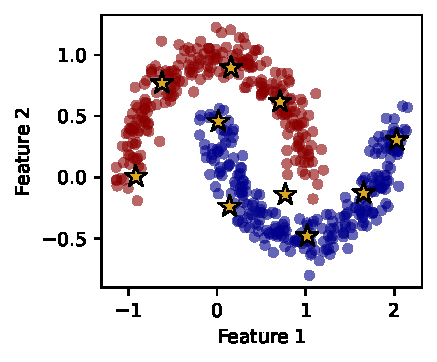
\includegraphics[height=6cm]{images/ssl/moon.pdf} % first figure
    \end{minipage}\hfill
    \begin{minipage}{0.44\textwidth}
        \centering
        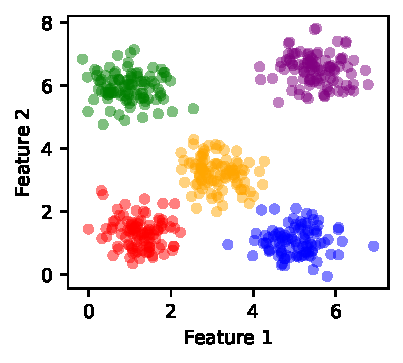
\includegraphics[height=6cm]{images/ssl/clusters.pdf} % second figure
    \end{minipage}
    \caption{Smoothness and cluster assumptions. \textbf{Left}: The moon dataset representing smoothness between 
        data points of each class. \textbf{Right}: The cluster assumption 
        illustrated with a toy example.}
    \label{fig:moon_cluster}
    \end{figure}

\begin{figure}[h]
    \centering
    \begin{minipage}{0.4\textwidth}
        \centering
        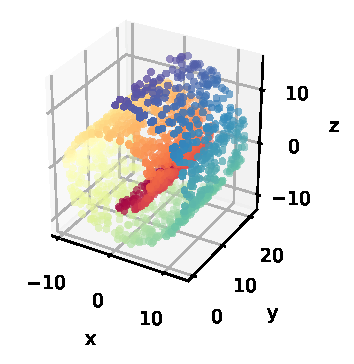
\includegraphics[height=6cm]{images/ssl/swiss_roll_3d.pdf} % first figure
    \end{minipage}\hfill
    \begin{minipage}{0.55\textwidth}
        \centering
        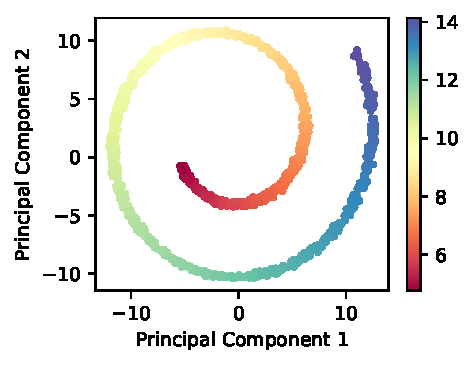
\includegraphics[height=6cm]{images/ssl/swiss_roll_pca.pdf} % second figure
    \end{minipage}
    \caption{Illustration of the manifold assumption. 
        \textbf{Left}: Data points are distributed in a high-dimensional space. 
        \textbf{Right}: The data points lie on a lower-dimensional manifold.}
    \label{fig:swiss_roll}
\end{figure}

\subsection{The Manifold Assumption}
\textbf{Assumption}: The data lies on a low-dimensional manifold embedded in a 
high-dimensional space.

This assumption is based on the idea that the data is not distributed uniformly 
in the input space, but it is concentrated on a lower-dimensional manifold.
It is fundamental to avoid problems related to the curse of dimensionality, 
which can lead to overfitting and poor generalization because of sparse data.

In Figure \ref{fig:swiss_roll}, the manifold assumption is illustrated with the 
Swiss roll dataset. The data points are distributed in a three-dimensional 
space, but they lie on a two-dimensional manifold. In general, the principal 
components analysis (PCA) can be used to reduce the dimensionality of the data, 
and in this specific case principal components are respectivlely the $x$ and $z$ 
axes.


\subsection{The Labeling Algorithm}
Classical pseudo-labeling methods usually train the teacher model on the labeled 
data and then they keep it fixed to predict the labels on the unlabeled data. 
The pseudo-labels are then used to train the student model, which is a copy of 
the teacher model. The student model is finally trained on the pseudo-labelled 
data.

On the other hand, on Meta Pseudo-Labels \cite{pham2021meta}, the teacher is 
trained along with the student model. In particular the student model is trained 
on the pseudo labels generated by the teacher model, and the teacher is trained 
on the performance of the student model on the labeled data. This process is 
repeated until the student model converges reaching a better performance 
with respect to the teacher. Therefore, the teacher model is updated to 
maximize the performance of the student.

In a more formal way, Pseudo Labels aims to optimize the student's 
loss function $CE(T(x_u, \theta_T), S(x_u, \theta_S))$, with the pseudo-labels 
generated from the teacher on the unlabeled data:

\begin{align}
    \theta_S^{PL} &= \arg \min_{\theta_S} \mathbb{E}_{x_u}\left[
        {CE(T(x_u, \theta_T), S(x_u, \theta_S))}\right] 
        \label{eq:pl_student_param}\\
        &:=
        \arg \min_{\theta_S} \mathcal{L}_u(\theta_T, \theta_S) \nonumber
\end{align}

where $T(x_u, \theta_T)$ is the pseudo target generated by the trained teacher 
model with its parameters $\theta_T$ already optimized and fixed. 
Therefore, the final goal of 
Pseudo Labels is to have a lower student loss with respect to the teacher on 
the labelled data:

\begin{align}
    \mathbb{E}_{x_l, y_l}\left[CE(y_l, S(x_l, \theta_S^{PL}))\right]
    &\leq
    \mathbb{E}_{x_l, y_l}\left[CE(y_l, T(x_l, \theta_T))\right]
    \qquad \Longleftrightarrow 
    \label{eq:pl_student_loss}\\
    \mathcal{L}_l(\theta_S^{PL})
    &\leq\
    \mathcal{L}_l(\theta_T) 
    \nonumber
\end{align}

Combining Equations (\ref{eq:pl_student_param}) and (\ref{eq:pl_student_loss}) 
it is possible to notice that the student loss $\mathcal{L}_l(\theta_S^{PL})$ 
depends on the teacher parameters $\theta_T$. Therefore, it could be possible 
get a better optimization of the teacher model to reduce the student loss. 
This is the main idea behind Meta Pseudo-Labels.
The final student loss $\mathcal{L}_l^*(\theta_S^{PL})$ will be the following:

\begin{align}
    \mathcal{L}^*_l(\theta_S^{PL*}) &= \min_{\theta_T} \mathcal{L}_l(\theta_S^{PL}(\theta_T))
    \label{eq:pl_student_loss_final} \\
    \text{where} \qquad \theta_S^{PL}(\theta_T) &= \arg\min_{\theta_S} \mathcal{L}_u(\theta_T, \theta_S)
\end{align}

However, the dependency of